\documentclass{article}
\usepackage[utf8]{inputenc}
\usepackage{graphicx}
\usepackage{hyperref}
\usepackage{amssymb}
\usepackage{float}

\title{Deep Learning Sentiment Analysis on Twitter Tweets}
\author{Md. Sakib Ibne Farhad, 012192004 \\
		Shakil Ahmed, 012203048 \\		
		CSE6211 (M): Deep Learning}
\date{\today}

\begin{document}

\maketitle
\begin{abstract}
    Twitter is the popular micro blogging site where thousands of people exchange their thoughts daily in the form of tweets that contain various types of sentiments. Our project focuses mainly on sentiment analysis of twitter data. We have built a model using LSTM that would be able to analyse a given piece of text and predicts whether this piece of text expresses positive or negative sentiment.
\end{abstract}

\section{Introduction} 
Social networks is a rich platform to learn about people’s opinion and sentiment regarding different topics as they can communicate and share their opinion actively on social medias including Facebook and Twitter. There are different opinion oriented information gathering systems which aim to extract people’s opinion regarding different topics. We are as of now over-burden with parts of unstructured information it gets to be exceptionally extreme to analyze the expansive volume of textual data. Sentiment analysis can be exceptionally valuable for businesses to label these texts. Sentimental Analysis can be done to compute feedback, reviews of the movies, etc. Opinion and sentimental mining has been well studied in this reference and all different approaches and research fields have been discussed\cite{liu2012sentiment}. The project aim is to explore Natural Language Processing (NLP) with Deep learning approach. Natural Language Processing (NLP) deals with actual text element processing. The text element is transformed into machine format by NLP. Artificial Intelligence (AI) uses information provided by the NLP and applies a lot of maths to determine whether something is positive or negative. Several methods exist to determine an author’s view on a topic from natural language textual information. 

Since social networks, especially Twitter, contains small texts and people may use different words and abbreviations which are difficult to extract their sentiment by current Natural Language processing systems easily, therefore some researchers have used deep learning and machine learning techniques to extract and mine the polarity of the text. Agarwal et al. (2011) \cite{agarwal2011sentiment} developed a 3-way model for classifying sentiment into positive, negative and neutral classes. They experimented with models such as: unigram model, a feature based model and a tree kernel based model.For tree kernel based model they represented tweets as a tree.The feature based model uses 100 features and the unigram model uses over 10,000 features. They arrived on a conclusion that features which combine prior polarity of words with their parts-of-speech(pos) tags are most important and plays a major rolein the classification task. The tree kernel based model outperformed the other two models. Pak and Paroubek(2010) \cite{pak2010twitter} proposed a model to classify the tweets as objective, positive and negative. They created a twitter corpus by collecting tweets using Twitter API and automatically annotating those tweets using emoticons. Using that corpus, they developed a sentiment classifier based on the multinomial Naive Bayes method that uses features like Ngram and POS-tags. The training set they used was less efficient since it contains only tweets having emoticons. Po-Wei Liang et.al.(2014) \cite{liang2013opinion} used Twitter API to collect twitter data. Their training data falls in three different categories (camera, movie , mobile). The data is labeled as positive, negative and non-opinions. Tweets containing opinions were filtered. Unigram Naive Bayes model was implemented and the Naive Bayes simplifying independence assumption was employed. They also eliminated useless features by using the Mutual Information and Chi square feature extraction method. Finally , the orientation of an tweet is predicted. i.e. positive or negative. Kouloumpis et al. \cite{kouloumpis2011twitter} explored the usefulness of various linguistic features for mining the sentiments of Twitter data. In this study, various feature sets were introduced using unigrams, bigrams, lexicons, micro-blogging and part-of-speech elements. The AdaBoost classifier was trained using these selected features in different combinations. The results showed that part-of-speech features were poor for sentiment analysis of Twitter data whilst micro-blogging features were the most useful. The best results were achieved
when n-gram features were employed alongside lexicon and micro-blogging features.
Balage Filho and Pardo \cite{ghiassi2013twitter} introduced a hybrid system for
detecting the sentiments present in tweets. Moreover, their system combined three classification methods: machine learning, rule-based, and lexicon-based. Balage Filho and Pardo \cite{ghiassi2013twitter} used the SentiStrength lexicon and the SVM
classifier as a machine learning method. The results obtained from the experiments showed that a hybrid system outperformed the individual classifiers, achieving an Fmeasure of 0.56 compared to 0.14, 0.448, and 0.49 obtained by the rule-based, lexicon-based, and SVM classifiers respectively.

The approach we are taking is unique because our training data was automatically created, as opposed to having humans manual annotate tweets. In our approach, we assume that any tweet with positive emoticons, like :), were positive, and tweets with negative emoticons, like :(, were negative. We used the Twitter Search API to collect these tweets by using keyword search.

\subsection{Our Contribution}
\begin{itemize}
  \item As we are using RNN, we do not need to select features manually.
  \item The created model can predict if a tweet has positive or negative sentiment.
\end{itemize}

\section{Material and Methods}
\begin{figure}[htp]
    \centering
    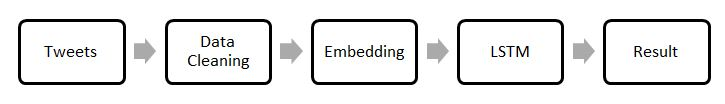
\includegraphics[width=10cm]{lstm.JPG}
    \caption{Block diagram of our project approach}
    \label{fig:galaxy}
\end{figure}
Initially, we will collect the data set. Then we will clean unnecessary words such as stopwords which do not hold any meaning useful to extract sentiment. After cleaning the data, we will use Word embeddings technique which is basically a way for us to convert words to representational vectors. By doing this, we will map each word to a vector of real numbers, representing this word, instead of mapping each word to an index. The goal here is to be able to generate similar or close representational vectors for words that have similar meaning. When word embeddings are done, we will build our model using LSTM and then train the data.

\subsection{Dataset Description}
We have used an existing data set called \textbf{Sentiment140}. Although it is not an open project, the corresponding data set is open for students. This is available from here:  \href{http://help.sentiment140.com/for-students/}{source}. and the download link: \href{http://cs.stanford.edu/people/alecmgo/trainingandtestdata.zip}{source}.

This zip file has 2 data set but we used the bigger data set that contains 1600000 training set. This CSV contains 6 fields. 

\begin{itemize}
    \item label
    \item time
    \item date
    \item query
    \item username
    \item text
\end{itemize}

\begin{figure}[h!]
    \centering
    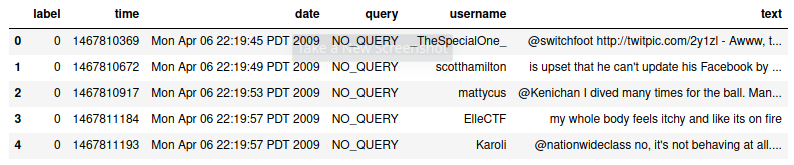
\includegraphics[width=12cm]{dataset.png}
    \caption{Data Set Table}
    \label{fig:dataset}
\end{figure}

For this simplification we used only label and text. As for hardware limitation we used 50,000 texts for our project which is $1/16$ of the total data. The labels from the data were 0 denotes Negative and 1 denotes Positive. For Tokenizations we used \href{https://www.nltk.org/api/nltk.tokenize.html#module-nltk.tokenize.casual}{twitter tokenizer}. The data was spitted into 2 parts, $90\%$ was for training and $10\%$ for testing.

we will use nltk\'s \href{https://www.ling.upenn.edu/courses/Fall_2003/ling001/penn_treebank_pos.html}{WordNetLemmatizer} to accomplish Lemmatization. This lemmatizer however takes as input two arguments: a list of tokens to be lemmatized as well as their corresponding part of speech. The most common parts of speech in English are nouns and verbs. In order to extract each token's part of speech, we will utilize nltk\'s post\_tag function, that takes an input a list of tokens, and returns a list of tuples, where each tuple is composed of a token and its corresponding position tag. Various position tags can be outputted from the pos\_tag function, however the most notable ones are:

\begin{itemize}
    \item \textbf{NNP}: Noun, Proper, Singular
    \item \textbf{NN}: Noun, Common, Singular or mass
    \item \textbf{VBG}: Verb, Gerund or Present Participle
    \item \textbf{VBN}: Vern, Past Participle
\end{itemize}


Word Clouds are one of the best visualizations for words frequencies in text documents.
Essentially, what it does is that it produces an image with frequently-appearing words in the text document, where the most frequent words are showcased with bigger font sizes, and less frequent words with smaller font sizes.

\begin{figure}[h!]
    \centering
    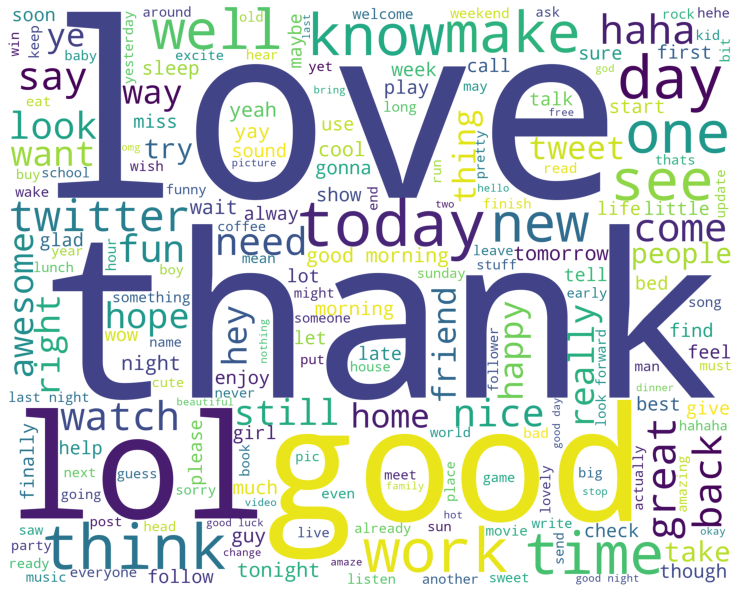
\includegraphics[width=10cm]{positive.png}
    \caption{Positive Words}
    \label{fig:positive_words}
\end{figure}


\begin{figure}[h!]
    \centering
    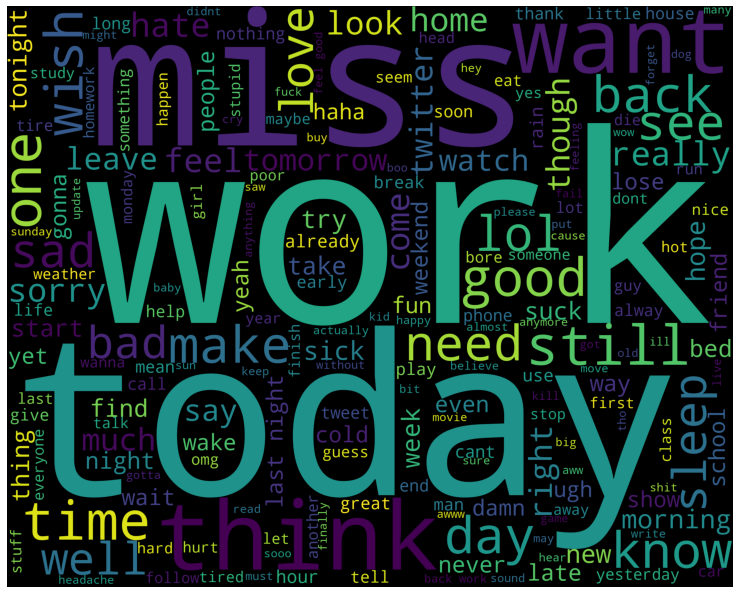
\includegraphics[width=10cm]{negative.png}
    \caption{Negative Words}
    \label{fig:negative_words}
\end{figure}

\newpage
\subsection{Neural Network Models / Algorithms Used}
After Cleaning out data set, we can use it to build our classification model. One of the most commonly used classification models in Natural Language Processing (NLP) is the Naive Bayesian.
Naive Bayesian classifiers are a collection of classification algorithms based on Bayes’ Theorem. It is not a single algorithm but rather a family of algorithms where all of them make the following naive assumptions:
\begin{itemize}
    \item All features are independent from each other.
    \item Every feature contributes equally to the output.
\end{itemize}

In our case, these two assumptions can be interpreted as:
\begin{itemize}
    \item Each word is independent from the other words, no relation between any two words of a given sentence.
    \item Each word contributes equally, throughout all sentences, to the decision of our model, regardless of its relative position in the sentence.
\end{itemize}
\textbf{Example}: "This is bad" / "This is very bad" or "Such a kind person" / "This kind of chocolate is disgusting", in both cases the Naive Bayesian classifier would give the same importance for the words 'bad' and 'kind', albeit them having a stronger meaning and a different meaning respectively in first and second sentences.

Nevertheless, Naive Bayesian are widely used in NLP and they often output great results.
The \textbf{Bayes\'  Theorem} describes the probability of an event $A$, based on prior knowledge of conditions $B$ hat might be related to the event: 

\begin{equation}
    P(A|B) = \frac{P(B|A)P(A)}{P(B)}  
\end{equation}

In our case, this can be intuitively interpreted as the probability of a tweet being positive, based on prior knowledge of the words inside the input text. In a nutshell, this probability is: the probability of the first word occuring in a positive tweet, times, the probability of the second word occuring in a positive tweet, ..., times, the probability of a tweet being positive. This can be mathematically written as: 

\begin{equation}
    P(A|B) \varpropto P(B_1|A) \times P(B_2|A) \times P(B_3|A) \times \cdots P(B_n|A) \times P(A)
\end{equation}

A \textbf{L}ong \textbf{S}hort-\textbf{T}erm \textbf{M}emory, or LSTM, is a type of machine learning neural networks. More specifically, it belongs to the family of Recurrent Neural Networds (RNN) in Deep Learning, which are specifically conceived in order to process temporal data. Temporal data is defined as data that is highly influenced by the order that it is presented in. This means that data coming before or after a given datum (singular for data) can greatly affect this datum. Text data is an example of temporal data. For example, let's consider the following sentence:

\textbf{Jane is not very happy. She's still mad at you!}

In the above sentence, the word not greatly influences the meaning of the upcoming words very happy. Also, we used the word she as we are speaking about a female subject.

Also, here's a fun example conveying the influence of words' positions directly influencing a sentence's meaning:

\textbf{Are you as clever as I am?}

\textbf{Am I as clever as you are?}

Further in our training we would like to speed the process up by splitting data into mini-batches. Batch learning is basically the process of training on several examples at the same time, which greatly decreases the training time!

However, and in order to be able to utilize batch learning, keras (and similarly to most machine learning frameworks) requires all data within the same batch to have the same length or dimension. Whereas in our text data, each example could have a variable sentence length. In order to overcome this issue, we will go over all of our data, and calculate the length of the longest phrase (in terms of words). Then, we will 0-pad all of the data sequences so that they will all have the same max\_len calculated.

Let's consider a max\_len of 5 words, and the two sentences I love you and I will be ready. First, we will convert these sentences to their corresponding index representation, then 0-pad them for the max\_len 5. After we've done that, we can now feed the resulting lists into a word embedding layer in order to get the representational vectors for each index:

\begin{figure}[h!]
    \centering
    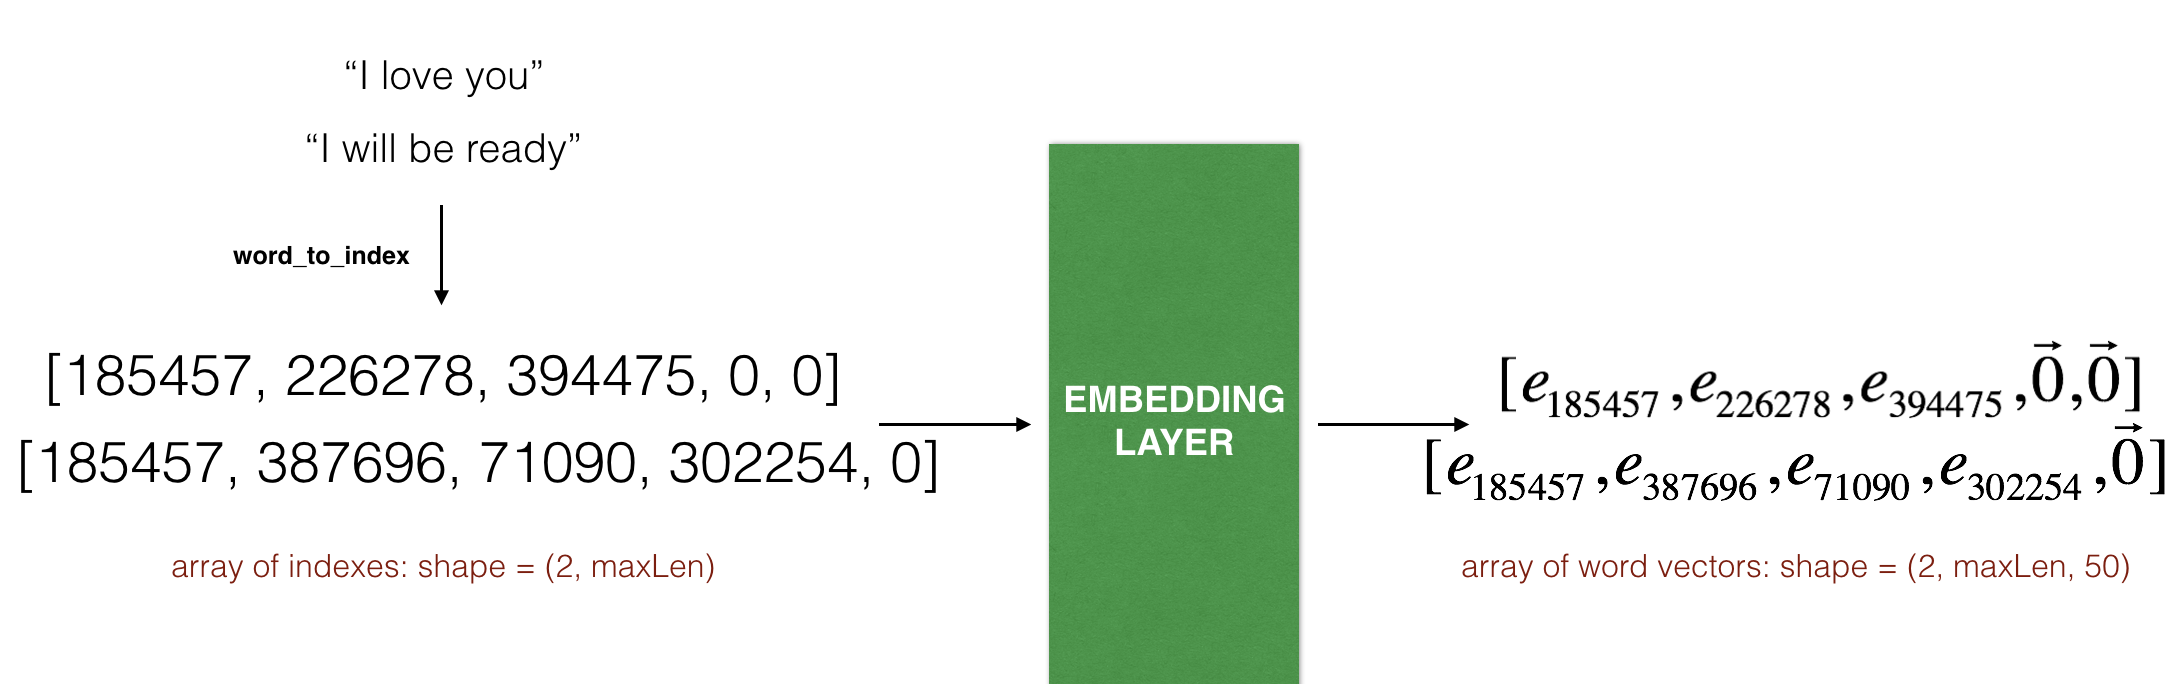
\includegraphics[width=10cm]{embedding.png}
    \caption{Embedding Model}
    \label{fig:my_label}
\end{figure}

Sequential model is given below:

\begin{figure}[h!]
    \centering
    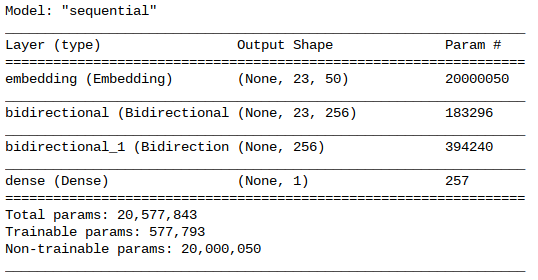
\includegraphics[width=10cm]{sequential.png}
    \caption{Sequential Model}
    \label{fig:sq_model}
\end{figure}

For loss function we used \textbf{binary\_crossentropy}, \textbf{adam} optimizer and \textbf{accuracy} matrics for compiling the model. 


\newpage
\subsection{Performance Evaluation}
The training accuracy is sky-rocketing, exceeding 95\% after 20 epochs! However, the validation accuracy increased slightly in the early epochs, reaching 76.6\% on the 6th epoch, after which it experienced a consistently gradual decrease. In data science, we would classify this model as having very high variance and low bias. This is also referred to as "over-fitting".

Over-Fitting is basically the phenomenon where the model's performance on validation data starts degrading, while still achieving great progress on the test set. In other words, the model is doing exceptionally well on learning specific examples it has been trained on, but is failing to generalize to data it never saw in its training phase.

Several directions could be undertaken at this stage in order to improve our model's performance. Arguably, the most promising direction to firstly look into is to introduce some kind of regularization in our model in order to try to reduce the clearly apparent over-fitting problem our model is facing. Let's specifically look at the dropout regularization technique.

\subsubsection{Regularization - Dropout}

\textbf{Regularization} is the process of preventing a model from over-fitting the training data. You can conceptualize regularization as being a tool we use in order to render our model less sensible to every detail, and possibly outliers, in the training data. This should allow the model to better generalize and have a better performance on the validation data, or any data it wasn't trained on.

\textbf{Dropout} is one of the many regularization techniques, and also one of the simplest to implement and most commonly used. Basically, what dropout does is that it randomly eliminates several (based on a parametrized percentage rate) neurons connections in the network, rendering the model less complex, and forcing the model to only look at part of a given example. The random elimination of connections in the model is repeated randomly for each example training data.

\begin{figure}[h!]
    \centering
    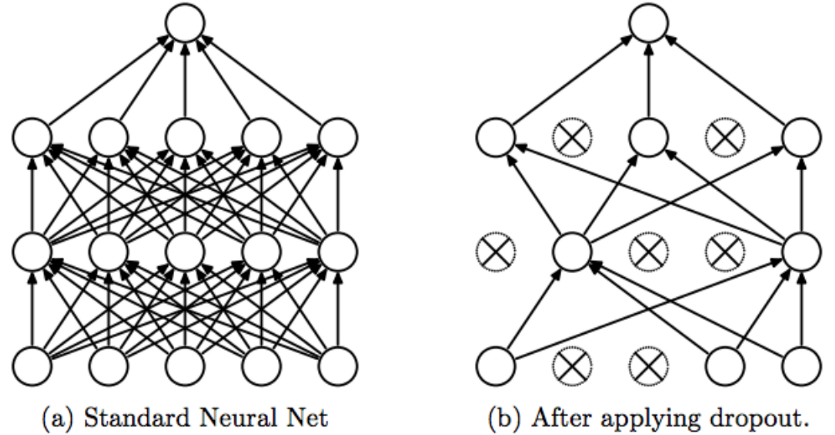
\includegraphics[width=10cm]{dropout.png}
    \caption{Dropout Model}
    \label{fig:my_label}
\end{figure}

For example, let's consider the following sentences, with a dropout layer with a rate of 0.5 (50% of connections will be eliminated):

\textbf{"Another kind of regularization can be directly applied to the cost function"}

\textbf{"This is my first ever notebook. Hope you're enjoying it so far!"}

The output of the dropout layer could look like the following:

\textbf{"kind of regularization be to function"}

\textbf{"This my notebook. you enjoying it far!"}

Thus, the model will only have information on a part of the input example, and should be able to escape over-fitting particular characteristics of the training data.

\begin{figure}[h!]
    \centering
    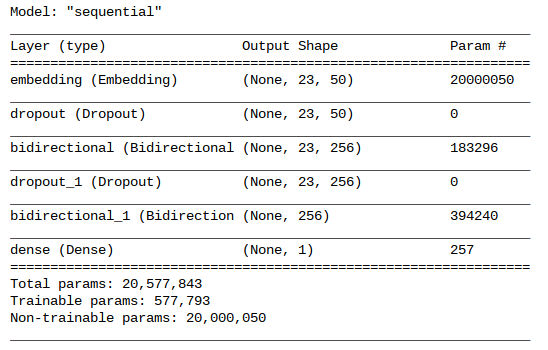
\includegraphics[width=10cm]{drop_seq.png}
    \caption{Drop Sequential Model}
    \label{fig:dsq_model}
\end{figure}

\newpage
\section{Experimental Analysis}
In order to feed our text data to our LSTM model, we'll have to go through several extra preprocessing steps.

Most neural networks expect numbers as inputs. Thus, we'll have to convert our text data to numerical data.

One way of doing so would be the following: collect all possible words in our dataset and generate a dictionary containing all unique words in our text corpus, then sort all of these words alphabetically and assign to each word an index. So for example, let's say our dictionary's length turned out to be 100,000 words. The word "a" would be assigned the index 0, the word "aaron" would be assigned the index 1, and so on, until we reach the last word in our dictionary, say "zulu", and assign to it the index 99,999. Great! Now each word is represented with a numerical value, and we can feed the numerical value of each word to our model.

It turns out that this step alone is not enough to be able to train good Deep Learning models. If you think about it, when the model reads an input 20,560 and then another input 20,561 for example, it would assume that these values are "close". However, those inputs could be the indexes of totally unrelated words, such as "cocktail" and "code", appearing right next to each other in the sorted dictionary. Hoping I've convinced you with this example, and that you hopefully believe that "cocktail" and "code" are, and should always be, completely unrelated, let's take a look at one solution that is widely adopted in various NLP implementations.

\newpage
Initial accuracy graph for our model:
\begin{figure}[h!]
    \centering
    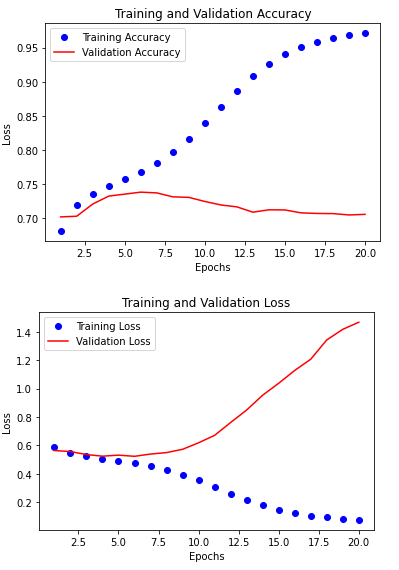
\includegraphics[width=8cm]{validation.png}
    \caption{Initial Training, Validation Accuracy and Loss}
    \label{fig:vg1_label}
\end{figure}

\newpage
Accuracy Graph after dropout
\begin{figure}[h!]
    \centering
    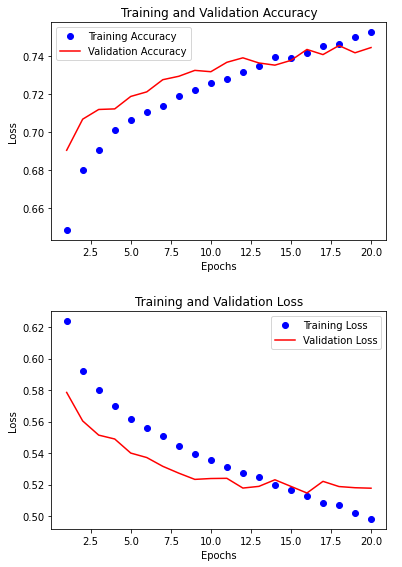
\includegraphics[width=8cm]{dropout_validation.png}
    \caption{Dropout Training, Validation Accuracy and Loss}
    \label{fig:vg1_label}
\end{figure}

\newpage
Accuracy loss graph with dropout
\begin{figure}[h!]
    \centering
    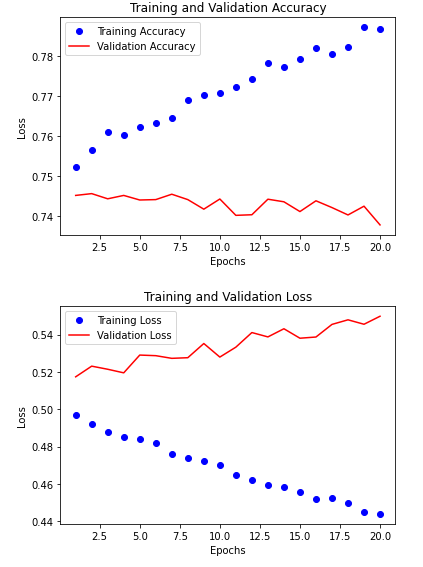
\includegraphics[width=8cm]{acc_validation.png}
    \caption{Dropout Training, Validation Accuracy and Loss}
    \label{fig:vg3_label}
\end{figure}

We can observe that the accuracy has plateaued, reaching its best validation value of 77.1\%.

Thus, we can conclude that the regularization process did not really help us in our case. A tiny 0.5\% improvement was observed after adding dropout to the model.

Project Source: \href{https://github.com/SakibFarhad/DeepLearningProject}{GitHub}

\section{Conclusion}
In this project, we build a model using LSTM that can figure out if a tweet has a positive sentiment or negative sentiment. Our model managed to reach an impressive 81\% validation accuracy. But in this project, we did not consider emoji into account. Moreover, we faced over-fitting problem that were persistent. In future work, we will further reduce over-fitting problem by introducing a more aggressive regularization and will train the model for a much bigger number of epochs, and will also train the model on a bigger, more diverse, cleaner data.

\bibliography{bibliography.bib}
\bibliographystyle{plain}
\end{document}